\documentclass{article}

\usepackage{amsmath, amsfonts, microtype, xcolor, tikz, graphicx, hyperref, amsthm}
\usepackage[ruled, linesnumbered]{algorithm2e}
\usepackage{iclr2020_conference,times,wrapfig}

\DeclareMathOperator*{\argmax}{argmax} % thin space, limits underneath in displays

\newtheorem{theorem}{Theorem}
\newtheorem*{theorem*}{Theorem}

\SetKwComment{Comment}{$\triangleright$\ }{}

\usetikzlibrary{calc}

\tikzset{
    ncbar angle/.initial=90,
    ncbar/.style={
        to path=(\tikztostart)
        -- ($(\tikztostart)!#1!\pgfkeysvalueof{/tikz/ncbar angle}:(\tikztotarget)$)
        -- ($(\tikztotarget)!($(\tikztostart)!#1!\pgfkeysvalueof{/tikz/ncbar angle}:(\tikztotarget)$)!\pgfkeysvalueof{/tikz/ncbar angle}:(\tikztostart)$)
        -- (\tikztotarget)
    },
    ncbar/.default=0.5cm,
}

\tikzset{round left paren/.style={ncbar=0.5cm,out=110,in=-110}}
\tikzset{round right paren/.style={ncbar=0.5cm,out=70,in=-70}}

\title{Measuring causal influence with\\ back-to-back regression: the linear case}

\author{%
  Jean-Remi King\\
  CNRS\\
  \texttt{jeanremi.king@gmail.com} \\
  \And
  Fran\c{c}ois Charton\\
  Facebook AI\\
  \texttt{fcharton@fb.com}\\
  \And
  David Lopez-Paz\\
  Facebook AI\\
  \texttt{dlp@fb.com}
  \And
  Maxime Oquab\\
  Facebook AI\\
  \texttt{qas@fb.com}
}

\begin{document}

\maketitle

\begin{abstract}
Identifying causes from observations can be particularly challenging when i) potential factors are difficult to manipulate individually and ii) observations are complex and multi-dimensional.
To address this issue, we introduce ``Back-to-Back'' regression (B2B), a
method designed to efficiently measure, from a set of co-varying factors, the causal
influences that most plausibly account for multidimensional observations. After
proving the consistency of B2B and its links to other linear approaches, we show that our method outperforms
least-squares regression and cross-decomposition techniques (e.g.
canonical correlation analysis and partial least squares) on causal
identification. Finally, we apply B2B to
neuroimaging recordings of 102 subjects reading word sequences. The results
show that the early and late brain representations, caused by low- and high-level
word features respectively, are more reliably detected with B2B than with other standard techniques.

\end{abstract}

\section{Introduction}

Natural sciences are tasked to find, from a set of hypothetical factors, the
minimal subset that suffices to reliably predict novel observations. This
endeavor is impeded by two major challenges.

First, causal and non-causal factors may be numerous and partially correlated.
% In physics,
% for example, one may be challenged to identify whether fusion is caused by a
% change in temperature or a change in pressure, as these two factors may, at
% first, be difficult to manipulate independently. This issue becomes increasingly
% pronounced as the number of potential factors increases.
In neuroscience, for
example, it can be challenging to identify whether word frequency modulates
brain activity during reading. Indeed, the
frequency of words in natural language covaries with other factors such as their
length (short words are more frequent than long words) and their categories
(determinants are more frequent than adverbs)
\citep{kutas2011thirty,pegado2014timing}. Instead of selecting a set of words
that controls for all of these factors simultaneously, it is thus common to use
a \emph{forward} "encoding model", i.e. to fit a linear regression to predict observations
(e.g. brain activity) from a minimal combination of competing factors (e.g.
word length, word frequency), and analytically investigate
the estimated contribution of each factor from the model's coefficients
\citep{friston1994statistical,naselaris2011encoding,weichwald2015causal,
king2018encoding,huth2016natural}.

The second challenge to measuring causal influence is that observations can be
multidimensional.
For example, brain activity is often
recorded with hundreds or thousands of simultaneous measurements via functional
Magnetic Resonance Imaging, magneto-encephalography (MEG) or multiple electro-
physiological probes \citep{friston1994statistical,steinmetz2018challenges}.
The relationship between putative causes and observations is thus often
done by training models in a \emph{backward}
fashion: i.e. from observations to putative causal factors. For example, it is
common to fit a support vector machine across multiple
brain voxels or multiple electrodes to detect the
category of a stimulus independently of common noise sources (e.g. head
movements, eye blink)
\citep{norman2006beyond,cichy2014resolving,
kriegeskorte2008representational, king2018encoding}.

Both \emph{forward} and \emph{backward} modeling have competing benefits and drawbacks.
Specifically, forward modeling disentangles the independent contribution of
correlated factors, but does not combine multidimensional observations. By
contrast, backward modeling combines multiple observations, but does not
disentangle factors that are linearly correlated \citep{weichwald2015causal,
hebart2018deconstructing, king2018encoding}. To combine some of the benefits of forward
and backward modeling, several authors have proposed to use cross-decomposition
techniques such as Partial Least Squares (PLS) and Canonical Correlation
Analysis (CCA) \citep{de2019multiway, bilenko2016pyrcca}. CCA and PLS aim to find, from two sets of
data $X$ and $Y$, the components $H$ and $G$ such that $XH$ and $YG$ are maximally
correlated or maximally covarying respectively.

While CCA and PLS can make use
of multidimensional features and observations, they are not designed
for feature discovery. First, these methods are not not directional: observations
and factors can be assigned to either $X$ or $Y$. Second, these method project $X$
and $Y$ onto a reduced but nonetheless multidimensional space. Third, because
CCA and PLS are based on a generalized eigen decomposition, their resulting
coefficients mix the features of $X$ and $Y$ in a way that makes them notoriously difficult to
interpret \citep{lebart1995statistique}.

Here, we introduce the `back-to-back regression' (B2B), which not only combines
the benefits of forward and backward modeling (Section~\ref{sec:algorithm}), but
can also provide robust, interpretable, unidimensional and unbiased coefficients for
each factor.

After detailing B2B and proving its convergence
(Section~\ref{sec:theorem}), we show with synthetic data that it outperforms
state-of-the-art forward, backward and cross-decomposition techniques in
disentangling causal factors (Section~\ref{sec:experiment_synthetic}). Finally,
we apply B2B to large neuroimaging datasets and reveal that distinct but
linearly-correlated word features lead to distinguishable brain representations
(Section~\ref{sec:experiment_real}).


\section{Back-to-Back regression}
\label{sec:algorithm}


\begin{figure}[t!]
    \centering
    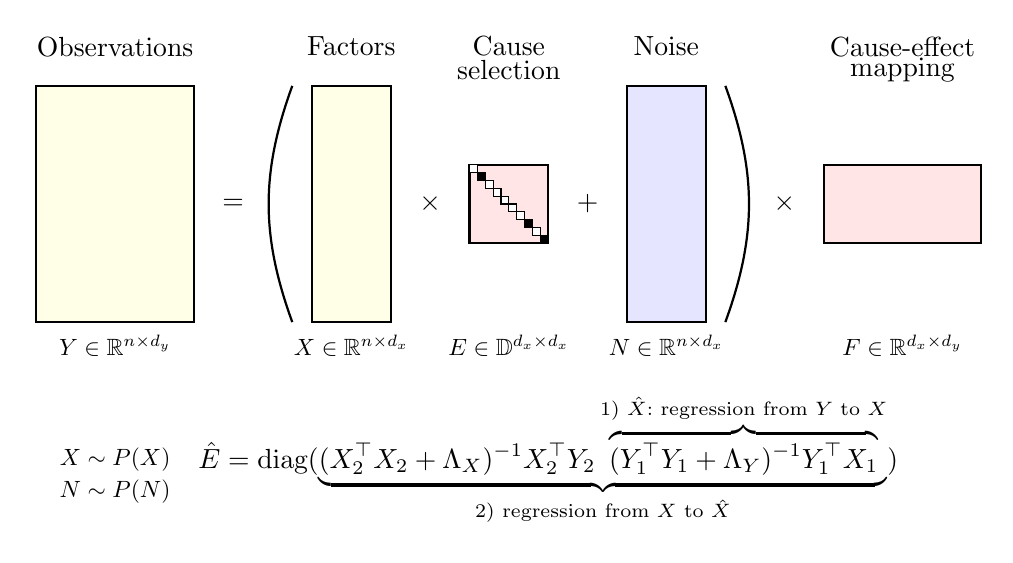
\begin{tikzpicture}
    \newcommand\posY{0}
    \newcommand\posX{3}
    \newcommand\posE{5}
    \newcommand\posN{7}
    \newcommand\posF{10}

    \node[thick, draw=black, minimum height=3cm, minimum width=2cm, fill=yellow!10] (Y) at (\posY, 0){};
    \node[] (eq) at (1.5, 0){$=$};
    \node[] (times) at (4, 0){$\times$};
    \node[thick, draw=black, minimum height=3cm, minimum width=1cm, fill=yellow!10] (X) at (\posX, 0){};
    \node[thick, draw=black, minimum height=1cm, minimum width=1cm, fill=red!10] (E) at (\posE, 0){};

    \draw[fill=white] (\posE - 0.5 + 0.0, 0.5 - 0.0) rectangle (\posE - 0.5 + 0.0 + 0.1, 0.5 - 0.0 - 0.1);
    \draw[fill=black] (\posE - 0.5 + 0.1, 0.5 - 0.1) rectangle (\posE - 0.5 + 0.1 + 0.1, 0.5 - 0.1 - 0.1);
    \draw[fill=white] (\posE - 0.5 + 0.2, 0.5 - 0.2) rectangle (\posE - 0.5 + 0.2 + 0.1, 0.5 - 0.2 - 0.1);
    \draw[fill=white] (\posE - 0.5 + 0.3, 0.5 - 0.3) rectangle (\posE - 0.5 + 0.3 + 0.1, 0.5 - 0.3 - 0.1);
    \draw[fill=white] (\posE - 0.5 + 0.4, 0.5 - 0.4) rectangle (\posE - 0.5 + 0.4 + 0.1, 0.5 - 0.4 - 0.1);
    \draw[fill=white] (\posE - 0.5 + 0.5, 0.5 - 0.5) rectangle (\posE - 0.5 + 0.5 + 0.1, 0.5 - 0.5 - 0.1);
    \draw[fill=white] (\posE - 0.5 + 0.6, 0.5 - 0.6) rectangle (\posE - 0.5 + 0.6 + 0.1, 0.5 - 0.6 - 0.1);
    \draw[fill=black] (\posE - 0.5 + 0.7, 0.5 - 0.7) rectangle (\posE - 0.5 + 0.7 + 0.1, 0.5 - 0.7 - 0.1);
    \draw[fill=white] (\posE - 0.5 + 0.8, 0.5 - 0.8) rectangle (\posE - 0.5 + 0.8 + 0.1, 0.5 - 0.8 - 0.1);
    \draw[fill=black] (\posE - 0.5 + 0.9, 0.5 - 0.9) rectangle (\posE - 0.5 + 0.9 + 0.1, 0.5 - 0.9 - 0.1);

    \node[] (plus) at (6, 0){$+$};
    \node[thick, draw=black, minimum height=3cm, minimum width=1cm, fill=blue!10] (N) at (\posN, 0){};
    \node[thick, draw=black, minimum height=1cm, minimum width=2cm, fill=red!10] (F) at (\posF, 0){};
    \draw [thick] (2.25, -1.5) to [round left paren ] (2.25, 1.5);
    \draw [thick] (7.75, -1.5) to [round right paren ] (7.75, 1.5);

    \node[] (times2) at (8.5, 0){$\times$};

    \node[] (annY) at (\posY, -1.8){\scalebox{0.85}{$Y \in \mathbb{R}^{n \times d_y}$}};
    \node[] (annX) at (\posX, -1.8){\scalebox{0.85}{$X \in \mathbb{R}^{n \times d_x}$}};
    \node[] (annE) at (\posE, -1.8){\scalebox{0.85}{$E \in \mathbb{D}^{d_x \times d_x}$}};
    \node[] (annN) at (\posN, -1.8){\scalebox{0.85}{$N \in \mathbb{R}^{n \times d_x}$}};
    \node[] (annF) at (\posF, -1.8){\scalebox{0.85}{$F \in \mathbb{R}^{d_x \times d_y}$}};

    \node[] (labY) at (\posY, 2){Observations};
    \node[] (labX) at (\posX, 2){Factors};
    \node[] (labE) at (\posE, 2){Cause};
    \node[] (labE) at (\posE, 1.7){selection};
    \node[] (labN) at (\posN, 2){Noise};
    \node[] (labF) at (\posF, 2){Cause-effect};
    \node[] (labF) at (\posF, 1.7){mapping};

    \node[] (sim1) at (0,-3.25) {\scalebox{0.85}{$X \sim P(X)$}};
    \node[] (sim2) at (0,-3.65) {\scalebox{0.85}{$N \sim P(N)$}};
    \node[] (reg1) at (5.5,-3.25) {$\hat{E} = \text{diag}(\underbrace{(X_2^\top X_2 + \Lambda_X)^{-1} X_2^\top Y_2\overbrace{(Y_1^\top Y_1 + \Lambda_Y)^{-1} Y_1^\top X_1}^{\text{1) } \hat{X} : \text{ regression from } Y \text{ to } X}}_{\text{2) regression from } X \text{ to } \hat{X}})$};
    \end{tikzpicture}
    \caption{Back-to-back regression identifies the subset of factors $E_{ii} = 1$ in $X$ that influence some observations $Y$ by 1) regressing from $Y$ to $X$ to obtain $\hat{X}$, and 2) returning the diagonal of the regression coefficients from $X$ to $\hat{X}$.}
    \label{fig:b2b}
\end{figure}

We consider the measurement of multivariate signal $Y \in \mathbb{R}^{n \times d_y}$, generated from a set of putative causes $X \in \mathbb{R}^{n \times d_x}$, via some unknown linear apparatus $F \in \mathbb{R}^{d_x \times d_y}$.
%
Not all the variables in $X$ exert a causal influence on $Y$.
%
By considering a square binary diagonal matrix of \emph{causal influences} $E \in \mathbb{D}^{d_x \times d_x}$, we denote by $XE$ the causal factors of $Y$.
%
In summary, the problem can be formalized as:
%
\begin{equation}
    y_i = (x_i E + n_i) F
    \label{eq:model}
\end{equation}
%
where $i$ is a given sample, and $n_i$ is a sample-specific noise drawen from a centered distribution.
%
While the triplet of variables $X$ and $N$ are independent, we allow each of them to have any form of covariance.
% what is a general covariance matrix?
%
In practice, we observe $n$ samples $(X, Y)$ from the model.
%
This problem space, along with the sizes of all variables involved, is illustrated in Figure~\ref{fig:b2b}.
%
Given the model in Equation~\eqref{eq:model}, \textbf{the goal} of Back-to-Back Regression (B2B) is to estimate the matrix of causal influences $E$.

\subsection{Algorithm}


Back-to-Back Regression (B2B) consists of two steps.
%
First, we estimate the linear regression coefficients $\hat G$ from $Y$ to $X$, and construct the predictions $\hat X = Y \hat G$.
%
This backward regression recovers the correlations between $Y$ and each factor of $X$.
%
Second, we estimate the linear regression coefficients $\hat H$ from $X$ to $\hat X$.
%
The diagonal of the regression coefficients $\hat H$, denoted by $\hat{E} = \text{diag}(\hat{H})$, is the desired estimate of the causal influence matrix $E$, as detailed in the \ref{appendix:theorem_proof}.

If using l2-regularized least-squares \citep{hoerl1959optimum, rifkin2007notes}, B2B has a closed form solution:
\begin{align}
    \hat G &= (Y^\top Y + \Lambda_Y)^{-1} Y^\top X,\label{eq:solG}\\
    \hat H &=(X^\top X + \Lambda_X)^{-1} X^\top Y \hat G,\label{eq:solH}
\end{align}
%
where $\Lambda_X$ and $\Lambda_Y$ are two diagonal matrices of regularization parameters, useful to invert the covariance matrices of $X$ and $Y$ if these are ill-conditioned.

Performing two regressions over the same data sample can result in overfitting, as spurious correlations in the data absorbed by the first regression will be leveraged by the second one.
%
To avoid this issue, we split our sample $(X, Y)$ into two splits $(X_1, Y_1)$ and $(X_2, Y_2)$.
%
Then, the first regression is performed using $(X_1, Y_1)$, and the second regression is performed using $(X_2, Y_2)$.
%
To compensate for the reduction in sample size caused by the split, B2B is repeated over many random splits, and the final estimate $\hat E$ of the causal influence matrix is the average over the estimates associated to each split \citep{breiman1996bagging}.
%
To accelerate this ensembling procedure, we implemented an efficient leave-one-out cross-validation scheme as detailed in \citep{rifkin2007notes} % http://cbcl.mit.edu/publications/ps/MIT-CSAIL-TR-2007-025.pdf
, as follows:
%

\begin{equation}
\hat{Y} = (\Sigma_X G Y - \text{diag}(\Sigma_X G) Y) \;/\; \text{diag}(I - \Sigma_X G) \qquad \text{(element-wise division)}
\end{equation}

where $\Sigma_X$ is the $X$ kernel matrix and where $G$ is computed with an eigen decomposition of $X$:
\begin{equation}
  \begin{aligned}
  \Sigma_X = Q V Q^T \\
  G = Q (V + \lambda I)^{-1} Q^T\\
  \end{aligned}
\end{equation}
where $Q$, $V$ and $\lambda$ are the eigen vectors, eigen values and regularization, respectively.

%
% After obtaining $\hat{E}$, we can fit a final regression from $X \hat{E}$ to $Y$.

We summarize the B2B procedure in Algorithm~\ref{algorithm:b2br}.
%
The rest of this section provides a theoretical guarantee on the correctness of B2B.


% JR: shall we update algorithm with LOO trick?
\begin{algorithm}[H]
    %\SetAlgoLined
    \KwIn{input data $X \in \mathbb{R}^{n \times d_x}$, output data $Y \in \mathbb{R}^{n\times d_y}$, number of repetitions $m \in \mathbb{N}$.}
    \KwOut{estimate of causal influences $\hat{E} \in \mathbb{D}^{d_x \times d_x}$.}
    $\hat{E} \leftarrow 0$\;
    \For{$i = 1, \ldots, m$}{
        $(X, Y) \leftarrow \text{ShuffleRows}((X, Y))$\;
        $(X_1, Y_1), (X_2, Y_2) \leftarrow \text{SplitRowsInHalf}((X, Y))$\;
        $\hat{G} = \text{LinearRegression}(Y_1, X_1)$ \Comment*[r]{$\hat G = (Y_1^\top Y_1 + \Lambda_Y)^{-1} Y_1^\top X_1$}
        $\hat{H} = \text{LinearRegression}(X_2, Y_2 \hat{G})$ \Comment*[r]{$\hat H=(X_2^\top X_2 + \Lambda_X)^{-1} X_2^\top Y_2 \hat G$}
        $\hat{E} \leftarrow \hat{E} + \text{diag}(\hat{H})$\;
    }
    $\hat{E} \leftarrow \hat{E} / m$\;
    $\hat{W} \leftarrow \text{LinearRegression}(X \hat{E}, Y)$\;
    \Return{$\hat{E}$, $\hat{W}$}
    \caption{Back-to-back regression.}
    \label{algorithm:b2br}
\end{algorithm}

\subsection{Theoretical guarantees}
\label{sec:theorem}

\begin{theorem}[B2B consistency - general case]

     Consider the B2B model from Equation $Y = (XE + N)F$, $N$ centred and full rank noise.
     %
     Let $Img(M)$ refers to the image of the matrix $M$. If $F$ and $X$ are full-rank on the $Img(E)$, then, the solution of B2B, $\hat H$, will minimize
     %
     $\min_H  \left \| X - XH\right\| ^2  + \left \| NH\right \| ^2$and satisfy $E\hat H = \hat H$
\end{theorem}
%
\begin{proof}
  See Appendix \ref{appendix:theorem_proof}.
\end{proof}

Since  $E\hat H = \hat H$, we have
\begin{equation}
  \hat H = \arg \min_H  \left \| X - XEH\right\| ^2  + \left \| NEH\right \| ^2 = (E X^\top XE +EN^\top NE) ^\dagger EXX^\top.
\end{equation}
% So, $\hat H = \arg \min_H  \left \| X - XEH\right\| ^2  + \left \| NEH\right \| ^2 = (E X^\top XE +EN^\top NE) ^\dagger EXX^\top$.

Assuming, without loss of generality, that the active features in $E$ are the $k \in \mathbb{Z}: k \in [0, d_x]$ first features, and rewriting $X=(X_1,X_2)$ and $N=(N_1,N_2)$ ($X_1$ and $N_1$ containing the $k$ first features), we have:

% $$
\begin{equation}
  X^\top X = \left(\begin{array}{lccl}\Sigma_{X_1 X_1} & \Sigma_{X_1 X_2} \\ \Sigma_{X_1 X_2} & \Sigma_{X_2 X_2}\end{array}\right),\qquad\qquad N^\top N = \left(\begin{array}{lccl}\Sigma_{N_1 N_1} & \Sigma_{N_1 N_2} \\ \Sigma_{N_1 N_2} & \Sigma_{N_2 N_2}\end{array}\right),
\end{equation}

where $\Sigma_{A B}$ is the covariance of $A$ and $B$, and:
% and
\begin{equation}
  \hat H = \left(\begin{array}{cc}(\Sigma_{X_1 X_1}+\Sigma_{N_1 N_1})^{-1}\Sigma_{X_1 X_1} & (\Sigma_{X_1 X_1}+\Sigma_{N_1 N_1})^{-1}\Sigma_{X_1 X_2} \\0 & 0\end{array}\right)
\end{equation}
\begin{equation}
  \text{diag}_k (\hat H) = \text{diag}((\Sigma_{X_1 X_1}+\Sigma_{N_1 N_1})^{-1}\Sigma_{X_1 X_1}) = \text{diag}((I+\Sigma_{X_1 X_1}^{-1}\Sigma_{N_1 N_1})^{-1})
  \label{eq:diagk}
\end{equation}
%
% $$
% $$
% $$
% $$
%
In the absence of noise, we have $\Sigma_{N_1 N_1}=0$, and so $\text{diag}_k(\hat H)=I$, and $$\text{diag}(\hat H) = \text{diag}(E)$$ Therefore, we recover $E$ from $\hat H$.


In the presence of noise, the causal factors of $E$ correspond to the positive elements of $\text{diag}(\hat H)$. The methods to recover them are presented in the Appendix \ref{recovering}.

\section{Experiments}

We perform two sets of experiments to evaluate B2B: one on controlled synthetic data, and a second one on a real, large-scale magneto-encephalography (MEG) dataset.
%
We use scikit-learn's PLS and RidgeCV \citep{sklearn} as well as pyrcca's regularized canonical component analysis (RegCCA, \citep{bilenko2016pyrcca}) objects to compare B2B against the standard baselines.

\subsection{Synthetic data}
\label{sec:experiment_synthetic}

We evaluate the performance of B2B throughout a series of experiments on
controlled synthetic data.
%
The purpose of these experiments is to evaluate the ability of B2B in terms of
prediction (inside and outside the training distribution), as well as a method
to recover causal factors.

The data generating process for each experiment constructs $n=1000$ training examples
according to the model $Y = (\text{snr} \cdot XE + N)F$, where $\text{snr}$ is a
scalar that modulates the signal-to-noise ratio.
%
Here,
%\begin{itemize} \item $F \in \mathbb{R}^{d_x \times d_y}$ contains entries
%drawn from $\mathcal{N}(0, d_x^{-1})$, \item $X \in \mathbb{R}^{n \times d_x}$
%contains rows drawn from $\mathcal{N}(0, \Sigma_X)$, \item $N \in \mathbb{R}^{n
%\times d_x}$ contains rows drawn from $\mathcal{N}(0, \Sigma_N)$, \item $E \in
%\mathbb{R}^{d_x \times d_x}$ is a binary diagonal matrix containing $n_c$ ones,
%\item $\Sigma_X = AA^\top$, where $A \in \mathbb{R}^{d_x \times d_x}$ contains
%entries drawn from $\mathcal{N}(0, d_x^{-1})$, \item $\Sigma_N = BB^\top$,
%where $B \in \mathbb{R}^{d_x \times d_x}$ contains entries drawn from
%$\mathcal{N}(0, d_x^{-1})$, \end{itemize}
    $F \in \mathbb{R}^{d_x \times d_y}$ contains entries drawn from
$\mathcal{N}(0, d_x^{-1})$, $X \in \mathbb{R}^{n \times d_x}$ contains rows
drawn from $\mathcal{N}(0, \Sigma_X)$, $N \in \mathbb{R}^{n \times d_x}$
contains rows drawn from $\mathcal{N}(0, \Sigma_N)$, $E \in \mathbb{R}^{d_x
\times d_x}$ is a binary diagonal matrix containing $n_c$ ones, $\Sigma_X =
AA^\top$ where $A \in \mathbb{R}^{d_x \times d_x}$ contains entries drawn from
$\mathcal{N}(0, d_x^{-1})$, $\Sigma_N = BB^\top$ where $B \in \mathbb{R}^{d_x
\times d_x}$ contains entries drawn from $\mathcal{N}(0, d_x^{-1})$, and the
factor $\text{snr} \in (0, \infty)$.

To simulate a wide range of experimental conditions, we sample 10 values in log-space for $d_x, d_y \in \left[ 10, 100 \right]$, $n_c \in \left[ 3, 63 \right]$,
$\text{snr} \in \left[ 0.001, 10 \right]$. We discard the cases where $n_c > d_x$, limit $d_x, d_y$ to 100 to keep the running time under 2 hours for each condition, and average over 5 random seeds.
%
% Each condition is simulated under $5$ different random seeds.

We compare the performance of B2B against four competing methods, all
implemented in scikit-learn \citep{sklearn}:
%
% To be updated

\subsection{Baseline models}

Forward regression consists of an $l2$-regularized "ridge" regression from the
putative causes $X$ to the observations $Y$: \begin{equation} H = (X^T X
+\lambda I)^{-1} X^T Y \end{equation}

Backward regression consists of an $l2$-regularized "ridge" regression from $Y$
to $X$: \begin{equation} G = (Y^T Y +\lambda I)^{-1} Y^T X \end{equation}

CCA finds $G\in\mathbb{R}^{d_z, d_y}$ and $H\in\mathbb{R}^{d_z, d_x}$
% such that
s.t.
$X$ and $Y$ are maximally correlated in a latent $Z$ space:
% \begin{equation} maxcorr(XH^T, YG^T) \end{equation}
\begin{equation} G,H = \argmax_{G,H} corr(XH^T, YG^T) \end{equation}

% To be checked
PLS finds $G\in\mathbb{R}^{d_z, d_y}$ and $H\in\mathbb{R}^{d_z, d_x}$
% such that
s.t.
$X$ and $Y$ are maximally covarying in a latent $Z$ space:
% \begin{equation} maxcov(XH^T, YG^T) \end{equation}
\begin{equation} G,H = \argmax_{G,H} cov(XH^T, YG^T) \end{equation}

We employ $5$-fold cross-validation to select the optimal number of components
for CCA and PLS. Regressions were $\ell2$-regularized with a $\lambda$ regularization
parameters fitted with the efficient leave-one-out procedure implemented in
scikit-learn RidgeCV \citep{sklearn}.

\subsection{Evaluating Causal Discovery from models' coefficients}

B2B leads to unbiased (i.e. zeros-centered) scalar coefficients for non-causal
features. In contrast, the Forward, Backward, CCA and PLS models lead to a
loading vector $H_i$ per feature $i$ (or one vector $G^i$ for the backward
model). To transform such vector into an estimated causal contribution $\hat E$,
we take the sum of square coefficients:
% \begin{equation}
  $\hat E_i = \sum_j {H^j_i}^2 $
% \end{equation}

To estimate whether models accurately identify causal factors, we compute the
area-under-the-curve (AUC) across factors $AUC(E, \hat E)$.
%\begin{equation} AUC = 1 - \sum_1^n (E_k - E_{k-1}) ( \hat{E}_k +
%\hat{E}_{k-1}) / 2 \end{equation}
The AUC allows evaluating the capacity of models at detecting the causal
importance of factors when ground truth labels are available, as is the case in
this setup.

We report AUC results in Figures~\ref{fig:percondition}~(top) and ~\ref{fig:auc_plots}~(left, in Appendix), and compare favorably to all baselines.

\begin{figure}[t]
  \centering
  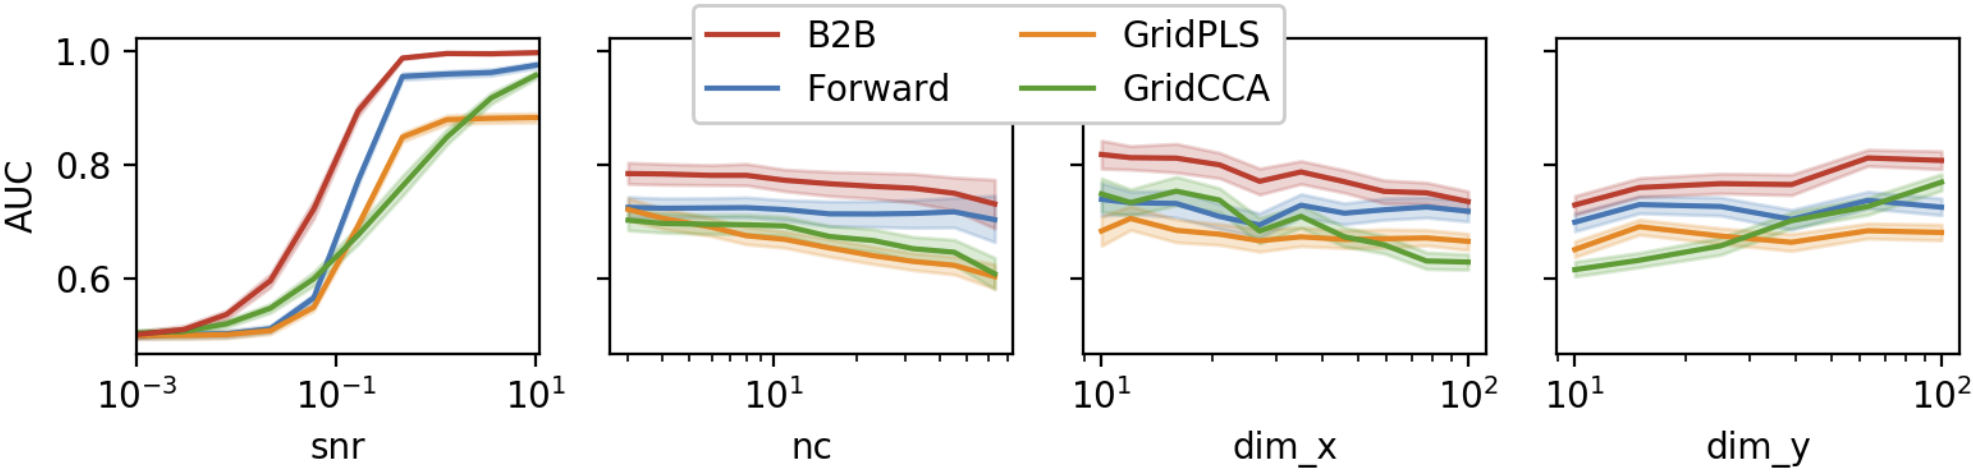
\includegraphics[width=\linewidth]{figures/AUC_conditions}
  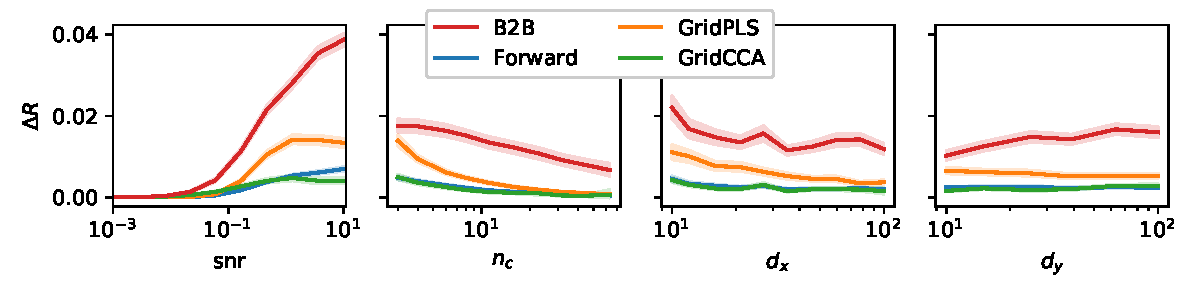
\includegraphics[width=\linewidth]{figures/R_conditions}
  \vspace{-4ex}
  \caption{Synthetic experiments. Average AUC (top) and Feature Importance $\Delta R$ (bottom) when varying experimental conditions individually. Higher is better. B2B compares favorably in all cases. \label{fig:percondition}}
\end{figure}


\subsection{Evaluating Causal Discovery with held-out prediction reliability}

In most cases, $E$ is not known and AUC can thus not be estimated.

To address this issue, we assess the ability of each model to reliably predict
independent and identically distributed data from $Y$, given all of the $X$
features versus all-but-ones feature $X_{-i}$ (i.e. 'knock-out X'). This procedure
results in two correlation metrics $R_{full}$ and $R_{knockout}$, whose
difference $\Delta R_i = R_{full}-R_{knockout}$ indicates how much each $X_i$
improves the prediction of $Y$.
%beyond what can be predicted from all other features $X_{-i}$.
In our figures, $\Delta R$ is the average of $\Delta R_i$. A higher score means that for prediction, the model relies on individual features rather than combinations of features.

We show in Appendix~\ref{appendix:feature_importance} pseudo-code to assess feature importance for our algorithm as well as baselines. For the Backward Model, feature importance cannot be assessed as there is no prediction.

% Feature importance can be computed similarly for the CCA, PLS and Forward baselines (see Appendix \ref{appendix:feature_importance}). For the Backward Model, feature importance cannot be assessed as there is no prediction.

We show in Figures~\ref{fig:percondition} (bottom) and \ref{fig:auc_plots} (right, in Appendix) that our method compares favorably to baselines.

%
% \iffalse
% For CCA and PLS, feature importance is assessed as follow:
% \begin{enumerate}
%   \item Fit $H$ and $G$ given $X_{train}$ and $Y_{train}$
%   \item For each feature $i$:
%   \begin{itemize}
%     \item Define $K$, and identity matrix whose row $i$ has been zeroed-out
%     \item Fit $H^i_k$ and $G_k$ given $X_{train} K$ and $Y_{train}$
%   \end{itemize}
% \end{enumerate}
% \fi
% For the Backward Model, feature importance cannot be assessed because there is no prediction.
% We thus simply
% report the model performance $R_i = corr(YG_i, X_i)$.


% \iffalse
% \begin{enumerate}
%
%   \item Fit $G$ given $X_{train}$ and $Y_{train}$
%   \item Fit $H$ given $X_{train}$ and $Y_{train} G^T$
%   \item For each feature $i$:
%   \begin{itemize}
%     \item Define $K$, and identity matrix whose row $i$ has been zeroed-out
%     \item Fit $H^i_k$ given $X_{train} K$ and $Y_{train} G^T$
%   \end{itemize}
%
%   \item Compute $R_{full}$ given $Y_{test} G^T$ and $X_{test}$
%   \item For all $i \in d_x$:
%   \begin{itemize}
%     \item Compute $R^i_{knockout}$ given $Y_{test} G^T$ and $X_{test} K {H^i_k}^T$
%     \item Compute $R^i_{delta}=R_{full} - R^i_{knockout}$
%   \end{itemize}
%   \end{enumerate}
% \fi

% \iffalse Ridge regression \citep{hoerl1959optimum}, multitask Lasso
% \citep{argyriou2008convex}, Partial Least Squares or PLS \citep{wold_pls,
% tenenhaus_pls}, Canonical Correlation Analysis or CCA \citep{cca_hotelling}, and
% Reduced Rank Regression or RRR \citep{Izenman_rrr}.
% %
% Each of these methods estimates a matrix of coefficients $\hat{W} \in
% \mathbb{R}^{d_x \times d_y}$, from which we estimate the diagonal mask $\hat{E}$
% using the feature importances $\hat{E}_{i,i} = \| W_{i, :} \|$.
% %
% For B2B, we obtain $\hat{E}$ as described in Algorithm~\ref{algorithm:b2br}.
% %
%
%
% We evaluate seven metrics:
% %
% test error in-distribution, test error out-distribution, test error-in
% distribution after weighting with $\hat{E}$, test error out-distribution after
% weighting with $\hat{E}$, Sonquist-Morgan false positives on $\hat{E}$,
% Sonquist-Morgan false negatives on $\hat{E}$, and the area under the ROC curve
% (AUC) between $\hat{E}$ and $E$.
% %
% The ``in-distribution'' metrics measure the test error of each predictor before
% and after weighting their features by the estimated (continuous!) mask
% $\hat{E}$.
% %
% The ``out-distribution'' metrics are similar, measuring the test error at
% samples drawn using two different random covariance matrices for both $X$ and
% $N$.
% %
% The false positives, false negatives, and AUC statistics measure the quality of
% identification of causal factors between $\hat{E}$ and the true, binary $E$.
%
% \begin{figure}[htpb] \centering
% 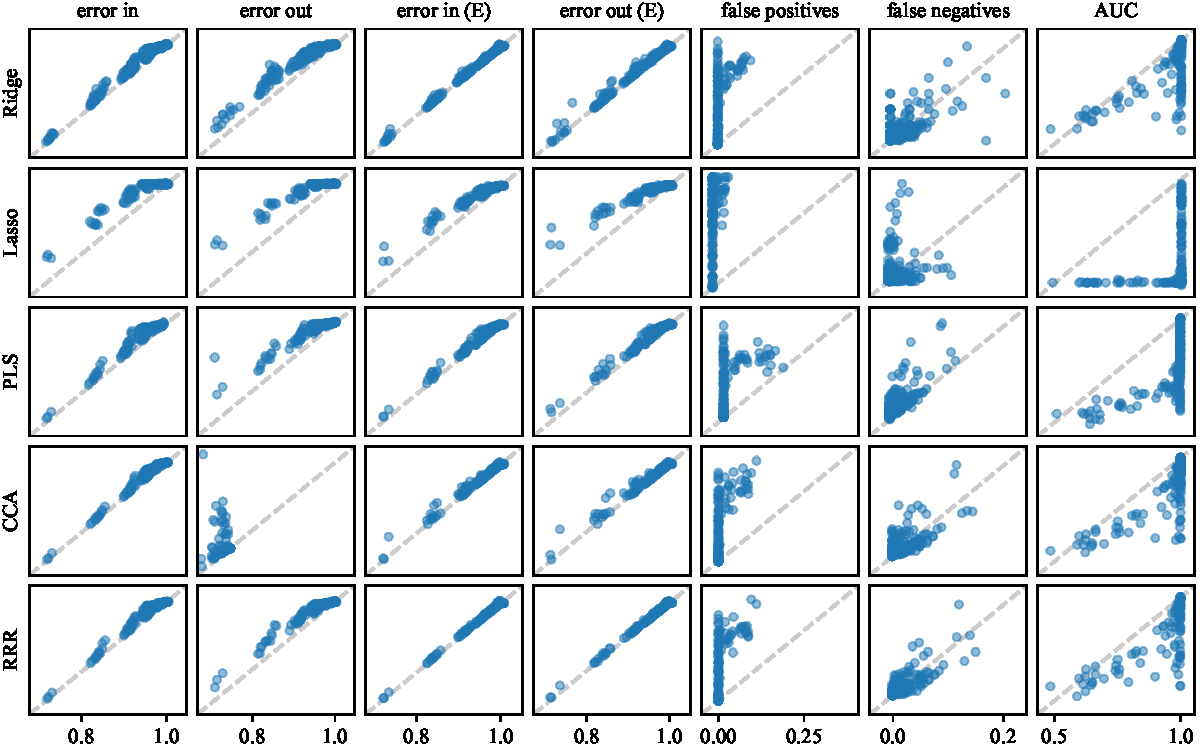
\includegraphics[width=\textwidth]{synthetic.pdf} \caption{Results of synthetic
% experiments. Each dot depicts the average value of a metric for B2B ($x$-axis)
% against a competitor ($y$-axis) for each experiment configuration averaged over
% $20$ random seeds. The prediction error on $Y$ within (in) and outside (out) of
% the training distribution are weakly but consistently larger for all of the
% models as compared to B2B with and without the Sonquist binarization (E). The
% AUC, measuring the ability of each model to separate causal from noncausal
% factors, is consistently larger in B2B as compared to the other models.}
% \label{table:synthetic} \end{figure} \fi

% Figure~\ref{table:synthetic} summarizes the results for all experimental
% conditions, metrics, and methods.
% %
% B2B is the method obtaining best test errors, lowest false positive and false
% negative discovery about $E$, and overall the best AUC when it comes to
% detecting causal influences.


\subsection{Magnetoencephalography data}
\label{sec:experiment_real}

%\newpage
%\subsection{Dataset}

Next, we apply our method to brain imaging data from the anonymized multimodal
neuroimaging ``Mother Of all Unification Studies'' (MOUS) dataset
\citep{schoffelen2019204}. The dataset contains magneto-encephalography (MEG)
recordings of 102 healthy native-Dutch adults who participated in a reading
task. Twelve subjects were excluded from the analysis because of corrupted file headers.
%
Subjects were exposed to a rapid serial visual presentation of Dutch words. The
word lists consisted of 120 sentences, and scrambled lists of the same words.
Each word was presented on the computer screen for 351ms on average (min: 300ms,
max: 1400ms). Successive words were separated by a blank screen for 300ms, and
successive sentences were separated by an empty screen for a few (3-4) seconds.

\subsubsection{MEG preprocessing}

The raw MEG data was bandpass-filtered between 0.1 and 40Hz using MNE-Python
default parameters \citep{gramfort2013meg, gramfort2014mne}. Specifically, we used a zero-phase finite impulse
response filter (FIR) with a Hamming window and with transition bands of 0.1Hz
and 10Hz for the low and high cut-off frequencies. The raw data was then segmented 100ms before word onset and 1s after
word onset ($t=0$ms corresponds to word onset). Finally, each resulting
segment was baseline-corrected between -100ms and 0ms, and decimated by 5 and
thus led a sampling frequency of 240Hz. The average responses across words is displayed in Figure \ref{fig:meg_evoked}.
For each subject and each time sample relative to word onset, we
build an observation matrix $Y \in \mathbb{R}^{n \times d_y}$ of $n\approx$ 2700 words
by $d_y=301$ MEG channels (273 magnetometers and 28 compensation channels). Each
of the columns of $Y$ is normalized to have zero mean and unit variance.

\begin{figure}[t!]
  \begin{minipage}[c]{0.6\textwidth}
    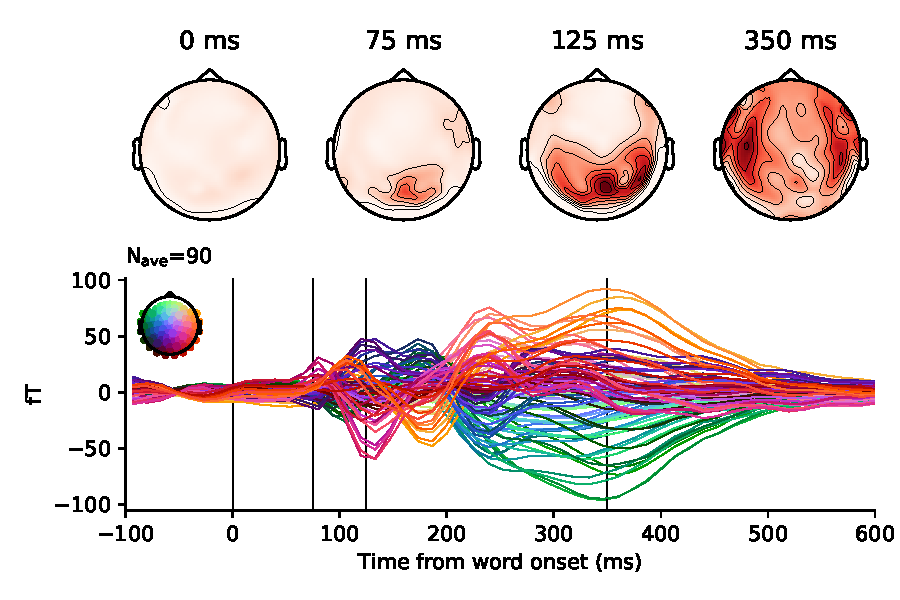
\includegraphics[width=\textwidth, trim=0cm 0cm 0cm 0cm, clip=True]{figures/meg_evoked.pdf}
  \end{minipage}\hfill
  \begin{minipage}[c]{0.4\textwidth}
    \caption{Ninety subjects read approximately 2,700 words while their brain activity was recorded with MEG. Top. Average brain response to words (word onset at t=0 ms), as viewed from above the head (red= higher gradient of magnetic flux). Bottom. Each line represents magnetometer, color-coded by spatial position. Posterior responses, typical of primary visual cortex activity, peak around 100 ms after word onset and are followed by an anterior propagation of activity typical of semantic processing in the associative cortices.
    }
    \label{fig:meg_evoked}
  \end{minipage}
\end{figure}


\subsubsection{Feature definition}

We aim to identify the word features that cause a variation in brain responses. We consider four distinct but colinear features.
%
First, 'Word Length' refers to the total number of letters. Word Length is expected to specifically cause a variation in the early evoked MEG responses (i.e. from 100 ms after stimulus onset) elicited by the retinotopically-tuned visual cortices (e.g. \citep{pegado2014timing}.).
%
Second, 'Word Frequency' indexes how frequently each word appears in Dutch and was derived with the the Zipf logarithmic scale of \citep{van2014subtlex} provided by the WordFreq package \citep{speerwordfreq}. Word Frequency is expected to specifically cause a variation in the late evoked MEG responses (i.e. from 400 ms), because it variably engages semantic processes in the temporal cortices \citep{kutas2011thirty}.
%
Third, 'Word Function' indicates whether each word is a content word (i.e. a noun, a verb, an adjective or an adverb) or a function word (i.e. a preposition, a conjunction, a determinant, a pronoun or a numeral), and was derived from Spacy's part of speech tagger \citep{spacy2}. To our knowledge, this feature has not been thouroughly investigated with MEG. Its causal contribution to reading processes in the brain thus remains unclear.
%
Finally, to verify that B2B and other methods would not inadequately identify non-causal features, we added a dummy feature, constructed from a noisy combination of Word Length and Word Frequency:
$dummy = z(length) + z(frequency) + \mathcal{N}$, where $z$ normalizes features and $\mathcal{N}$ is a random vector sampling Gaussian distribution (all terms thus have a zero-mean and a unit-variance).

This procedure yields an $X \in \mathbb{R}^{n \times d_x}$ matrix of $n\approx$ 2700 words by
$d_x=4$ features for each subject. Each of the columns of $X$ is normalized to
have a mean and a standard deviation of 0 and 1 respectively.

\subsubsection{Models and statistics}

We compare B2B to four standard methods: Forward regression, Backward regression, CCA and PLS, as implemented in scikit-learn \citep{sklearn}, and optimized with nested cross validation over twenty $l2$ regularization parameters logarithmically spaced between $10^{-4}$ and $10^4$ (for regression methods) or 1 to 4 canonical components (for cross-decomposition methods).

We used the feature importance described in Algorithm \ref{algorithm:b2b_fi} to assess the extent to which each feature $X_i$ specifically improves the prediction of held-out $Y$ data, using a 5-fold cross-validation.

Each model was implemented for each subject and each time sample independently. Pairwise comparison between models were performed using a Wilcoxon test across subjects (n=90) using the average $\Delta R$ across time.

Corresponding results are shown in Figure~\ref{fig:meg_results}.



\begin{wrapfigure}{r}{.5\textwidth}
  \vspace{-12ex}
  \begin{center}
    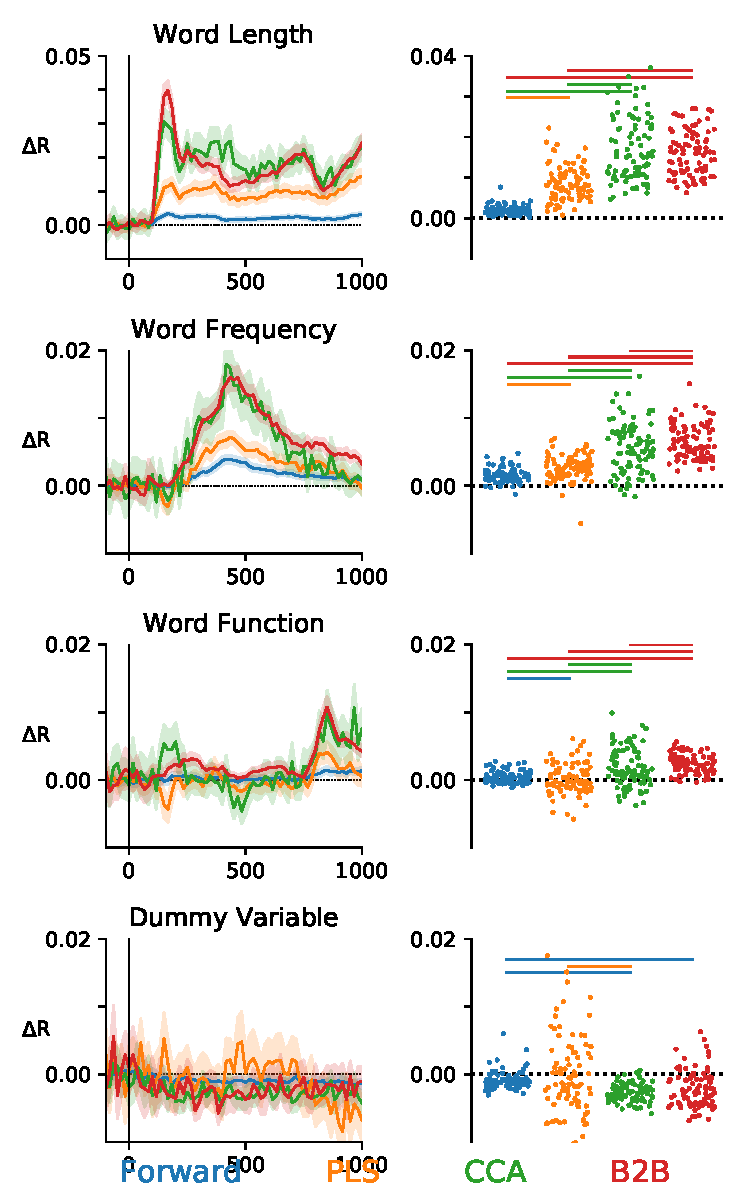
\includegraphics[width=0.48\textwidth, trim=0cm 0cm 0cm 0cm, clip=True]{figures/meg.pdf}

    \label{fig:meg_results}
  \end{center}
  \caption{Multiple models (color-coded) are compared on their ability to reliably predict single-trial MEG signals evoked by words. Left. Average improvement of correlation coefficient $\Delta R$ for each of the four features (rows). Error bars indicate standard error of the mean (SEM) across subjects. Right. Average $\Delta R$ across time for each subject (dot). Top horizontal lines indicate when B2B significantly outperforms other methods.}
  \vspace{-9ex}
\end{wrapfigure}

\subsubsection{Results}
We compared the ability of Forward regression, Backward regression, CCA, PLS and B2B to estimate the causal contribution of four distinct but collinear features on brain evoked responses to words.

Supplementary Figure \ref{fig:meg_supp} shows that the Backward model decodes the dummy variable well above chance level. In addition, the Backward model reveal a similar decoding time course for Word Length and Word Frequency, even though these features are known to specifically influence early and late MEG responses respectively \citep{kutas2011thirty}. These results illustrate that backward modelling cannot be used to estimate the causal contribution of collinear features.

We thus focus on the four remaining methods (i.e. Forward Regression, PLS, CCA, and B2B) and estimate their $\Delta R$ (i.e. the improvement of Y prediction induced by the introduction of a given feature into the model \ref{algorithm:b2b_fi}). Contrary to the Backward Model, none of the models predicted the Dummy Variable to improve the $Y$ prediction: all $\Delta R < 0$ (all $p > .089$).

Figure \ref{fig:meg_results} shows, for each model, the effects obtained across time (left) and subjects (right).

Word Length and Word Frequency improved the prediction performance of all methods: $\Delta R>0$ for all models (all $p<0.0001$). As expected, the time course associated with Word Length and Word Frequency rose from $\approx$ 100 ms and from $\approx$ 400 ms respectively. Furthermore, Word Function improved the prediction performance of all models (all $p < 0.0002$) except for PLS~($p=0.7989$). Overall, these results confirm that Word Length, Word Frequency and Word Function causally influence specific periods of brain responses to words.

To assess which model would be most sensitive to these causal discoveries, we compared B2B to other models across subjects (Figure \ref{fig:meg_results} right). For Word Length B2B outperforms all models (all $p < 0.00001$) but CCA ($p=0.0678$). For Word Frequency, B2B outperforms all models (all $p < 0.0006$). For "Word Function", B2B outperforms all models (all $p < 0.0015$). Overall, these results show that B2B reliably outperform standard methods, especially when the effects are difficult to detect.


\section{Related work}

Forward and cross-decomposition models have been used to identify the causal contribution of collinear features onto multi-dimensional observations (e.g. \citep{naselaris2011encoding}). These approaches typically lead to multiple coefficients for each features (i.e. one per dimension of $Y$ or one per component respectively). Furthermore, these coefficients can be difficult to summarize into a single causal estimate. By contrast, B2B quickly (Fig. \ref{fig:duration}) leads to a single unbiased scalar values $\hat E$ tending towards 1 and 0 for causal and non-causal features respectively.

A variety of other statistical methods applied to neuroimaging data have been proposed to clarify what is being represented in brain responses - i.e. what feature causes specific brain activity. One of the popular linear method is Representational Similarity Analysis (RSA) \citep{kriegeskorte2008representational}, and consists in analyzing the similarity of brain responses associated with specific categorical conditions (e.g. distinct images), by (1) fitting one-against-all classifiers on each condition and (2) testing whether these classifiers can discriminate all other conditions. The resulting confusion matrix is then analyzed in an unsupervised manner to reveal which conditions lead to similar brain activity patterns. B2B differs from RSA in that (1) it uses regressions instead of classifications, and can thus generalize to new items and new contexts and (2) it is fully supervised.

Finally, CCA has been used in neuroimaging for a variety of purposes such as denoising and subject alignment \citep{cca_hotelling, de2019multiway}. While CCA relates to B2B, these two methods diverge in several ways.
First, CCA and B2B have different objectives: CCA aims to find the potentially numerous and poorly interpretable components where X and Y are maximally correlated, whereas B2B aims to recover the causal factors from X to Y.
Second, B2B is not symmetric between $X$ and $Y$: it aims to identify specific causal features by first optimizing over the decoders $G$ and then over $H$. By contrast, CCA is symmetric between $X$ and $Y$, and aims to find $G$ and $H$ such that they project $X$ and $Y$ on maximally correlated dimensions.
Third, CCA is based an eigen decomposition of $XH$ and $YG$ - the corresponding canonical components are thus mixing the $X$ features in way that limit interpretability and potentially dilute the impact of each feature onto multiple components. In contrast B2B assesses each feature $X^j$ on a single $Y$ component specifically selected to maximize signal-to-noise ratio of that feature $j$. Fourth, and unlike B2B, CCA does not separately optimize two distinct regularization parameters for $G$ and $H$.
Finally, CCA does not use different data splits to estimate $G$ and $H$.
Together, these differences may explain why B2B reliably outperform CCA on estimating causal influences (Figs. \ref{fig:percondition} and \ref{fig:auc_plots}).

% I find a bit surprising to mention cauaslity literare in ML at the end. I would have expected this in the introduction to convince reviewer that know your stuff.



\section{Conclusion}
In this work, we proposed Back-to-Back Regression (B2BR), a method to 
measure the causal influence of a potential set of variables generating some observations.
%
B2BR performs two successive multidimensional regressions: one from the output domain, and another one from the input domain.
%
We provided a theoretical guarantee about the consistency of B2BR, and compared it to several baselines in controlled synthetic experiments.
%
We also applied B2BR to a recent brain imaging dataset, analyzing the timing
of brain responses and their connection to word features.
%
We obtained results consistent with prior work in neuroscience literature, confirming the efficacy of B2BR for real data analysis.


\clearpage
\newpage

\bibliographystyle{iclr2020_conference}
\bibliography{paper}

% \documentclass{article}

\usepackage{amsmath, amsfonts, microtype, xcolor, tikz, graphicx, hyperref, amsthm}
\usepackage[ruled, linesnumbered]{algorithm2e}
\usepackage[]{neurips_2019}
\newtheorem{theorem}{Theorem}


\title{Measuring causal influence with\\ back-to-back regression: the linear case - supplementary material}

\begin{document}

\appendix

\maketitle


\section{Theorem - detailed proof}
\label{sec:theorem}

\begin{theorem}[B2B consistency - general case]

     Consider the B2B model from Equation $$Y = (XS + N)F$$ $N$ centered and full rank noise.

     If $F$ and $X$ are full-rank on $Img(S)$, then, the solution of B2B, $\hat H$, will minimize

     $$\min_H  \left \| X - XH\right\| ^2  + \left \| NH\right \| ^2$$ and satisfy

     $$S\hat H = \hat H$$
\end{theorem}
\begin{proof}

 Let $\hat G$ and $\hat H$ be the solutions of the first and second regressions of B2B.

 Since $\hat G$ is the least square estimator of $X$ from $Y$
 \begin{align*}
    \hat G = \arg \min_G \mathbb{S}[\left \| YG - X \right \|^2]
\end{align*}
Replacing $Y$ by its model definition $Y = (XS+N)F$, we have
 \begin{align*}
    \hat G &=   \arg \min_G \mathbb{S}[\left \| X - (XS + N)FG \right\|^2] =\arg \min_G \mathbb{S}[\left \| X - XSFG + NFG \right\|^2]
  \end{align*}
  Since $N$ is centered and independent of $X$, we have
  \begin{align}
    	  \hat G &=  \arg \min_G \left \| X - XSFG\right\| ^2  + \left \| NFG\right \| ^2
     \label{eq:Gdoublenorm}
\end{align}

Samely, for $\hat H$, we have
\begin{align*}
    \hat H = \arg \min_H \mathbb{S}[\| XH - Y \hat{G} \|^2] &=\arg  \min_H \mathbb{S}[\| XH - (XS + N)F \hat G \|^2] \\
    &=\arg \min_H \mathbb{S}[\| X(H - SF \hat G) \| ^2] + \mathbb{S}[\| NF\hat G \| ^2]\\
    &= \arg \min_H \mathbb{S}[\| X(H - SF \hat G) \| ^2]
 \end{align*}
 a positive quantity which reaches a minimum (zero) for
 \begin{align}
    \hat H = SF \hat G
    \label{eq:Hdoublenom}
\end{align}

Let us now prove that $SF\hat G = F\hat G$.

Let $F^\dagger$ be the pseudo inverse of $F$, and $Z=F^\dagger SF\hat G$, we have $FZ = FF^\dagger SF \hat G$

Since $F$ is full rank on $Img(S)$, we have $FF^\dagger S =S$, and $FZ = SF\hat G$

As $S$ is a binary diagonal matrix, it is an orthogonal projection and therefore a contraction, thus
 $$ \| NSF\hat G\|^2 \leq \| NF\hat G \|^2$$ and
 $$\left \| X - XSFZ\right \| ^2  + \left \| NFZ\right \| ^2 = \| X - XSF\hat G \| ^2  + \| NSF\hat G \| ^2 \leq \| X - XSF\hat G \| ^2  + \| NF\hat G \| ^2$$

But since $\hat G =  \arg \min_G \left \| X - XSFG\right\| ^2  + \left \| NFG\right \| ^2$, we also have
$$\left \| X - XSF\hat G\right\| ^2  + \left \| NF\hat G\right \| ^2 \leq \left \| X - XSFZ\right \| ^2  + \left \| NFZ\right \| ^2$$

Summarizing the above,
$$\left \| X - XSF\hat G\right\| ^2  + \left \| NF\hat G\right \| ^2 \leq \| X - XSF\hat G \| ^2  + \| NSF\hat G \| ^2 \leq \| X - XSF\hat G \| ^2  + \| NF\hat G \| ^2$$
$$\left \| X - XSF\hat G\right\| ^2  + \left \| NF\hat G\right \| ^2 = \| X - XSF\hat G \| ^2  + \| NSF\hat G \| ^2$$
$$\left \| NF\hat G\right \| ^2 =  \| NSF\hat G \| ^2$$

$N$ being full rank, this yields $SF\hat G = F\Hat G$.

Replacing into $\eqref{eq:Gdoublenorm}$, and setting $H = SFG$, we have
\begin{align*}
	\hat G &=  \arg \min_G  \left \| X - XSFG\right \| ^2  + \left \| NFG\right \| ^2 \\
	&=   \arg \min_G \left \| X - XSFG\right \| ^2  + \left \| NSFG\right \| ^2 \\
	\hat H &=  \arg \min_H \left \| X - XH\right \| ^2  + \left \| NH\right \| ^2
	\label{eq:4}
\end{align*}

Finally, $S\hat H = S SF\hat G = SF\hat G = \hat H$, since $S$, a binary diagonal matrix, is involutive. This completes the proof.
\end{proof}



\end{document}


%\section{Appendices}
%
%This should hold part of the tests, explanations on simulation, detailed results and stuff on meg data

\newpage
\appendix
\section{Appendix}

\subsection{Proof of consistency theorem}
\label{appendix:theorem_proof}

Proof of the theorem in \ref{sec:theorem}:


\begin{theorem}[B2B consistency - general case]

     Consider the B2B model from Equation $$Y = (XE + N)F$$ $N$ centred and full rank noise.

     If $F$ and $X$ are full-rank on $Img(E)$, then, the solution of B2B, $\hat H$, will minimise

     $$\min_H  \left \| X - XH\right\| ^2  + \left \| NH\right \| ^2$$ and satisfy

     $$E\hat H = \hat H$$
\end{theorem}
\begin{proof}

 Let $\hat G$ and $\hat H$ be the solutions of the first and second regressions of B2B.

 Since $\hat G$ is the least square estimator of $X$ from $Y$
 \begin{align*}
    \hat G = \arg \min_G \mathbb{E}[\left \| YG - X \right \|^2]
\end{align*}
Replacing $Y$ by its model definition $Y = (XE+N)F$, we have
 \begin{align*}
    \hat G &=   \arg \min_G \mathbb{E}[\left \| X - (XE + N)FG \right\|^2] =\arg \min_G \mathbb{E}[\left \| X - XEFG + NFG \right\|^2]
  \end{align*}
  Since $N$ is centered and independent of $X$, we have
  \begin{align}
    	  \hat G &=  \arg \min_G \left \| X - XEFG\right\| ^2  + \left \| NFG\right \| ^2
     \label{eq:Gdoublenorm}
\end{align}

Samely, for $\hat H$, we have
\begin{align*}
    \hat H = \arg \min_H \mathbb{E}[\| XH - Y \hat{G} \|^2] &=\arg  \min_H \mathbb{E}[\| XH - (XE + N)F \hat G \|^2] \\
    &=\arg \min_H \mathbb{E}[\| X(H - EF \hat G) \| ^2] + \mathbb{E}[\| NF\hat G \| ^2]\\
    &= \arg \min_H \mathbb{E}[\| X(H - EF \hat G) \| ^2]
 \end{align*}
 a positive quantity which reaches a minimum (zero) for
 \begin{align}
    \hat H = EF \hat G
    \label{eq:Hdoublenom}
\end{align}

Let us now prove that $EF\hat G = F\hat G$.

Let $F^\dagger$ be the pseudo inverse of $F$, and $Z=F^\dagger EF\hat G$, we have $FZ = FF^\dagger EF \hat G$

Since $F$ is full rank on $Img(E)$, we have $FF^\dagger E =E$, and $FZ = EF\hat G$

As $E$ is a binary diagonal matrix, it is an orthogonal projection and therefore a contraction, thus
 $$ \| NEF\hat G\|^2 \leq \| NF\hat G \|^2$$ and
 $$\left \| X - XEFZ\right \| ^2  + \left \| NFZ\right \| ^2 = \| X - XEF\hat G \| ^2  + \| NEF\hat G \| ^2 \leq \| X - XEF\hat G \| ^2  + \| NF\hat G \| ^2$$

But since $\hat G =  \arg \min_G \left \| X - XEFG\right\| ^2  + \left \| NFG\right \| ^2$, we also have
$$\left \| X - XEF\hat G\right\| ^2  + \left \| NF\hat G\right \| ^2 \leq \left \| X - XEFZ\right \| ^2  + \left \| NFZ\right \| ^2$$

Summarizing the above,
$$\left \| X - XEF\hat G\right\| ^2  + \left \| NF\hat G\right \| ^2 \leq \| X - XEF\hat G \| ^2  + \| NEF\hat G \| ^2 \leq \| X - XEF\hat G \| ^2  + \| NF\hat G \| ^2$$
$$\left \| X - XEF\hat G\right\| ^2  + \left \| NF\hat G\right \| ^2 = \| X - XEF\hat G \| ^2  + \| NEF\hat G \| ^2$$
$$\left \| NF\hat G\right \| ^2 =  \| NEF\hat G \| ^2$$

$N$ being full rank, this yields $EF\hat G = F\Hat G$.

Replacing into $\eqref{eq:Gdoublenorm}$, and setting $H = EFG$, we have
\begin{align*}
	\hat G &=  \arg \min_G  \left \| X - XEFG\right \| ^2  + \left \| NFG\right \| ^2 \\
	&=   \arg \min_G \left \| X - XEFG\right \| ^2  + \left \| NEFG\right \| ^2 \\
	\hat H &=  \arg \min_H \left \| X - XH\right \| ^2  + \left \| NH\right \| ^2
	\label{eq:4}
\end{align*}

Finally, $E\hat H = E EF\hat G = EF\hat G = \hat H$, since $E$, a binary diagonal matrix, is involutive. This completes the proof.
\end{proof}



\newpage
\subsection{Feature importance}
\label{appendix:feature_importance}

For B2B, feature importance is assessed as follows:

\begin{algorithm}[H]
    %\SetAlgoLined
    \KwIn{$X_{train} \in \mathbb{R}^{n \times d_x}$, $X_{test} \in
\mathbb{R}^{n' \times d_x}$, $Y_{train} \in \mathbb{R}^{n\times d_y}$, $Y_{test}
\in \mathbb{R}^{n'\times d_y}$, } \KwOut{estimate of prediction improvement
$\Delta{R} \in \mathbb{D}^{d_x}$.} $H, G = \text{B2B}(X_{train}, Y_{train})$\;
$R_{full} = \text{corr}(X_{test} H, Y_{test} G)$\;

    \For{$i = 1, \ldots, d_x$}{ $K = Id$\; $K[i] \leftarrow 0$\;
    $R_{k} =
\text{corr}(X_{test} K H, Y_{test} G_i)$\; $\Delta R_i = R_{full} - R_{k}$\; }
\Return{$\Delta R$} \caption{B2B feature importance.} \label{algorithm:b2b_fi}
\end{algorithm}

For the Forward Model, the feature importance is assessed as follows:

\begin{algorithm}[H]
    %\SetAlgoLined
    \KwIn{$X_{train} \in \mathbb{R}^{n \times d_x}$, $X_{test} \in
\mathbb{R}^{n' \times d_x}$, $Y_{train} \in \mathbb{R}^{n\times d_y}$, $Y_{test}
\in \mathbb{R}^{n'\times d_y}$, } \KwOut{estimate of prediction improvement
$\Delta{R} \in \mathbb{D}^{d_x, d_y}$.}

$H = \text{LinearRegression}(X_{train}, Y_{train})\;
R_{full} = \text{corr}(X_{test} K, Y_{test})$\;

    \For{$i = 1, \ldots, d_x$}{ $K = Id$\; $K[i] \leftarrow 0$\; $R_{k} = \text{corr}(X_{test}
K H, Y_{test})$\; $\Delta R_i = R_{full} - R_{k}$\; } \Return{$\Delta R$}
\caption{Forward feature importance.} \label{algorithm:fwd_fi} \end{algorithm}

% \iffalse
% \begin{enumerate}
%   \item Fit $H$ given $X_{train}$ and $Y_{train}$
%   \item For each feature $i$:
%   \begin{itemize}
%     \item Define $K$, and identity matrix whose row $i$ has been zeroed-out
%     \item Fit $H^i_k$ given $X_{train} K$ and $Y_{train}$
%   \end{itemize}
%   \end{enumerate}
% \fi

For the CCA and PLS models, the feature importance is assessed as follows:

\begin{algorithm}[H]
    %\SetAlgoLined
    \KwIn{$X_{train} \in \mathbb{R}^{n \times d_x}$, $X_{test} \in
\mathbb{R}^{n' \times d_x}$, $Y_{train} \in \mathbb{R}^{n\times d_y}$, $Y_{test}
\in \mathbb{R}^{n'\times d_y}$, } \KwOut{estimate of prediction improvement
$\Delta{R} \in \mathbb{D}^{d_x, d_z}$.} $H, G = \text{CCA}(X_{train},
Y_{train})$\; $R_{full} = \text{corr}(X_{test} H, Y_{test} G)$\;

    \For{$i = 1, \ldots, d_x$}{ $K = Id$\; $K[i] \leftarrow 0$\; $R_{k} = \text{corr}(X_{test} K H,
Y_{test} G)$\; $\Delta R_i = R_{full} - R_{k}$\; } \Return{$\Delta R$}
\caption{CCA and PLS feature importance.} \label{algorithm:cdp_fi}
\end{algorithm}

For the Backward Model, feature importance cannot be assessed because there is no prediction.

\subsection{Binarizing $\hat{H}$ - the Sonquist-Morgan criterion}

Back to back regression provides us with $Diag(\hat{H})$, a vector of real numbers that estimate the causal influence of features in $X$. In order to derive the true causal influence matrix $E$ , a binary matrix, we need to binarize  $\hat{H}$, i.e. test each feature for equality with zero. In regression analysis, the traditional approach to this problem employs a $t$-test to check whether the regression coefficients differ from zero \citep{student1908probable}. This test will not succeed here: $\hat{H}$ is obtained from a double regression with regularization, and will not follow the t-distribution.

Instead, we treat the binarization of $\hat{H}$ as a clustering problem: separate the elements in the diagonal into a group of ``small values'', and a group of ``large values''. More specifically, we propose to maximize the ratio of inter-group variance and to minimize the intra-group variance, over all possible splits of the diagonal into $p$ largest values and $d_x-p$ smallest values.
%
Letting $m_0$ and $m_1$ be the average values of the two clusters, $p$ and $d_x-p$ their size, and $v$ the total variance of the sample, we select the split maximizing the Sonquist-Morgan \citep{sonquist_morgan} \citep{kass75} criterion $\frac{p(d_x-p)}{d_x} \frac{(m_1 - m_0)^2}{v}$.
%
To binarize $\hat{H}$, set to one all the $p$ diagonal entries belonging to the ``large values'' group in the decided split, and setting to zero the rest of the $d_x-p$ diagonal entries.


\section{Additional Figures}


% \begin{figure}[t!]
%   \centering
%   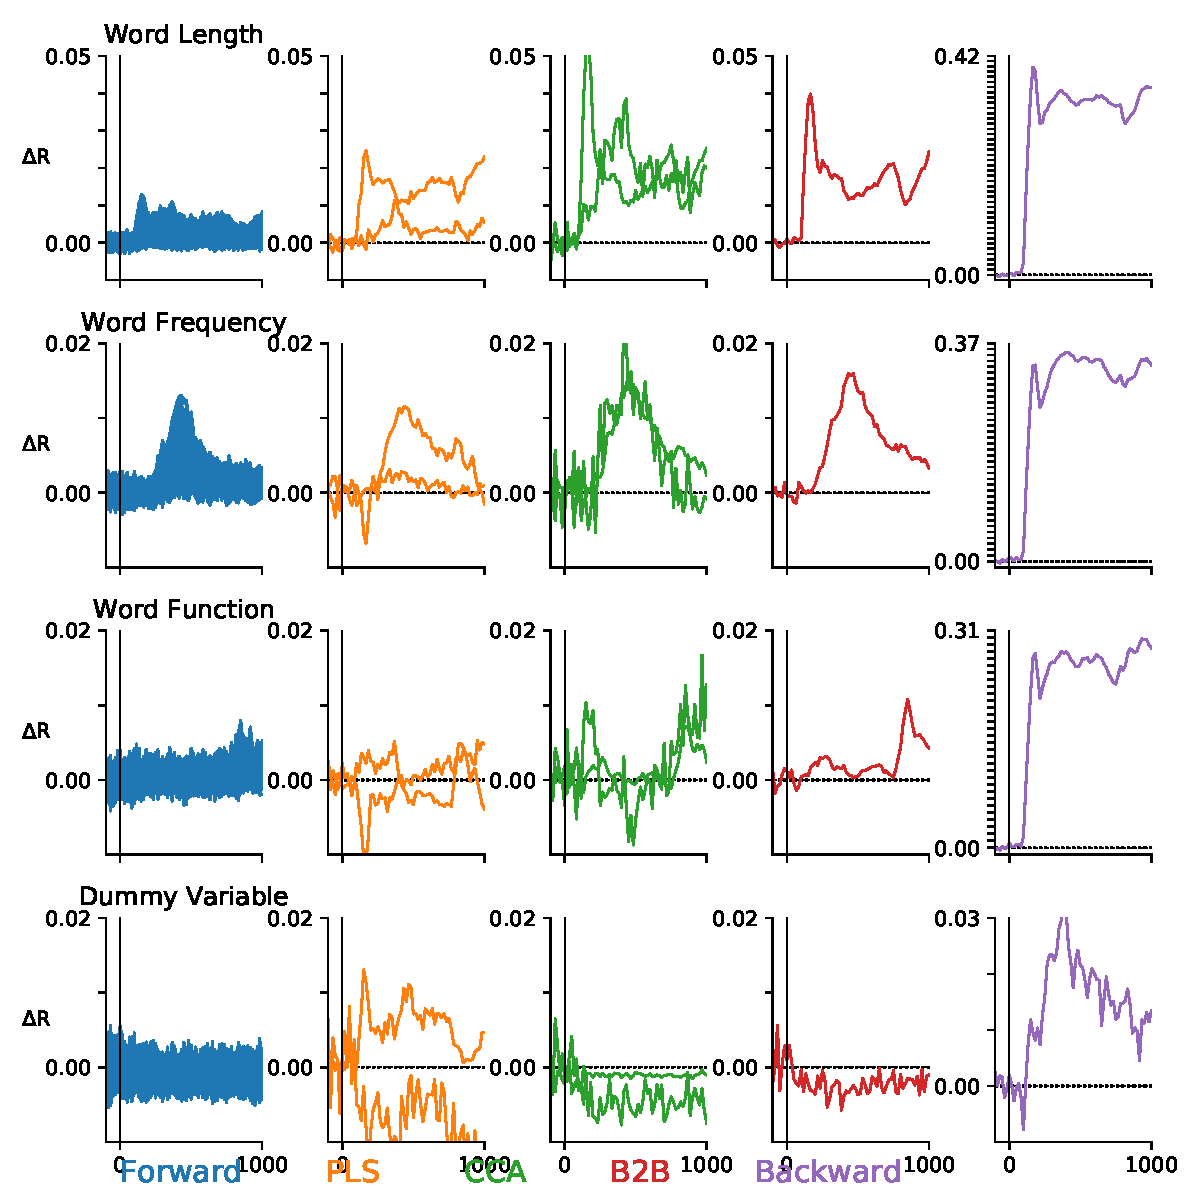
\includegraphics[width=\textwidth, trim=0cm 0cm 0cm 0cm, clip=True]{figures/meg_supp.pdf}
%   \caption{Average $\Delta R$ for each $Y$ dimension (Forward model), canonical components (PLS and CCA) or feature (B2B) across subjects. Formally, Backward model cannot have a $\Delta R$ because it never unmixes the multiple $X$ features. In such cases, we thus simply report the decoding score.}
%   \label{fig:meg_supp}
% \end{figure}


\begin{figure}
  \centering
  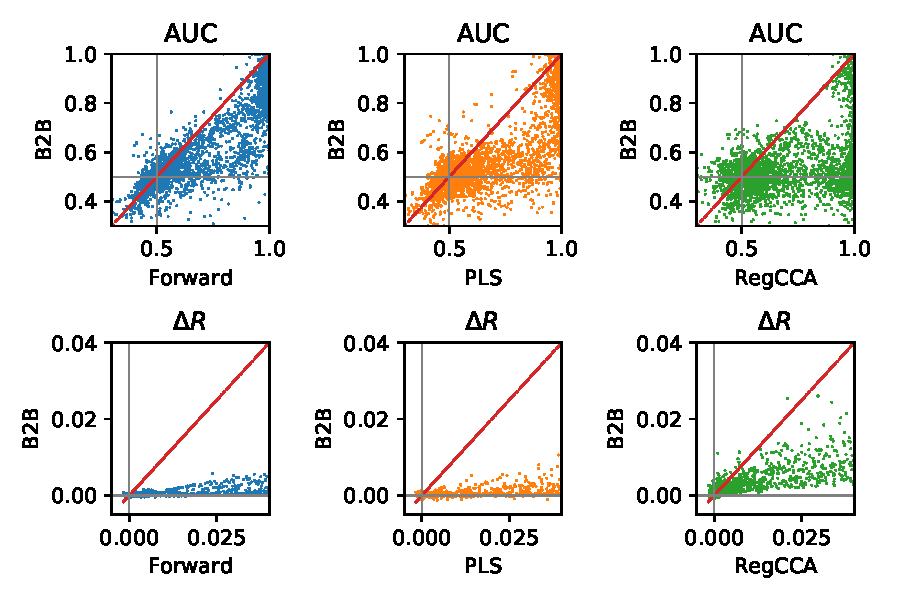
\includegraphics[width=\linewidth]{figures/delta_auc.pdf}
  \caption{Synthetic experiments. Distribution (over conditions) of AUC (top) and Feature Importance $\Delta R$ (bottom) metrics between our method (y-axis) and the baselines (x-axis). Each dot is a distinct synthetic experiment. Dots below the diagonal indicates that B2B outperform the tested model. \label{fig:auc_plots}}
\end{figure}

\begin{figure}
  \centering
  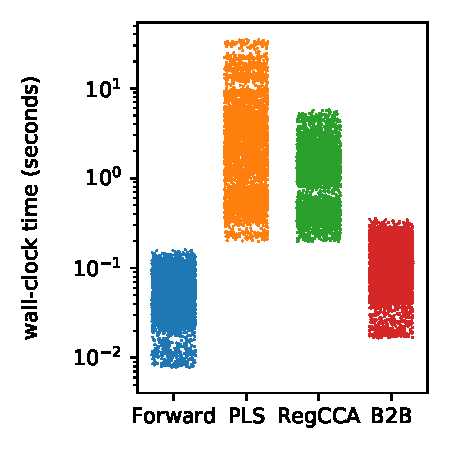
\includegraphics[width=0.7\linewidth]{figures/duration}
  \caption{Wall-clock run-time for our method B2B and for the baselines. Each dot is a distinct synthetic experiment. B2B runs much faster than cross-decomposition baselines. \label{fig:duration}}
\end{figure}


\subsection{Robustness on increasing number of factors}

To test whether each of the methods robustly scale to an increasingly large number of potential causes $X$, we enhance the four ad-hoc features (word length, word frequency, word function, dummy variable) with another ten features. These additional features corresponds to the first dimensions of word embedding as provided by Spacy \citep{spacy2}. The results shown in Figure \ref{fig:embbeding}, show that the ad-hoc features remain unchanged (and are actually improved) in the B2B.

\begin{figure}
  \centering
  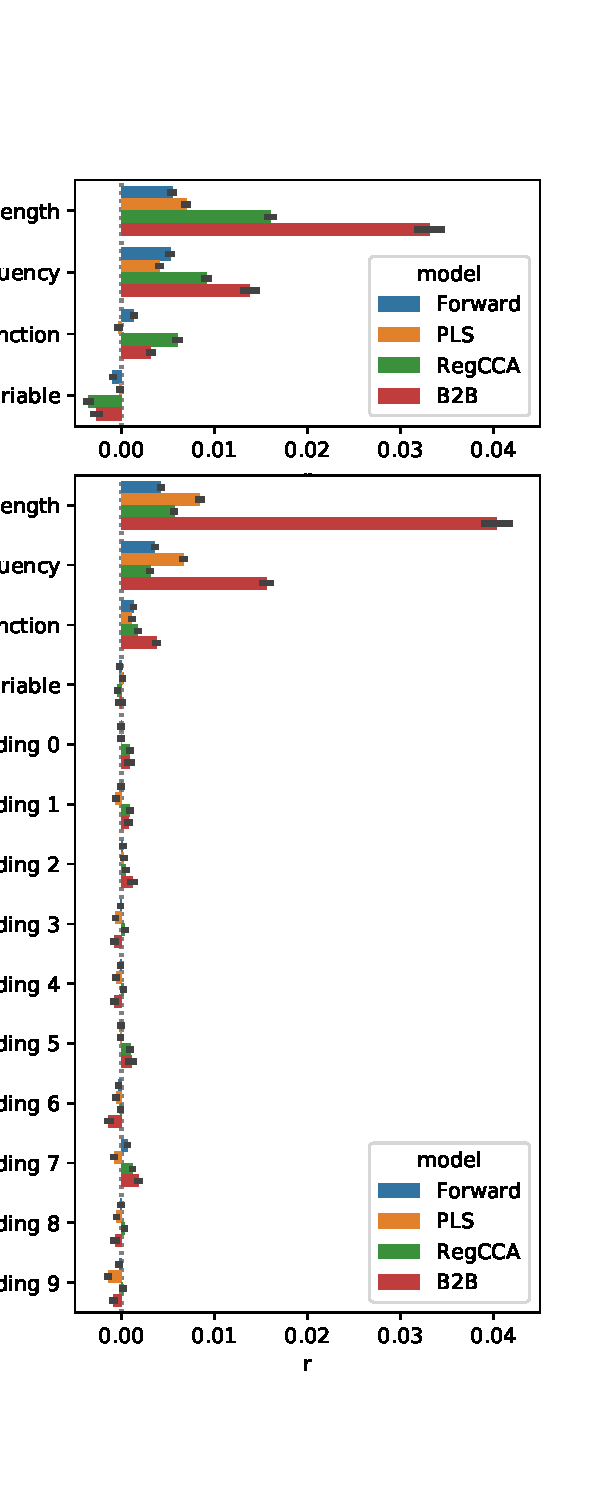
\includegraphics[width=0.7\linewidth]{figures/compare_embeddings.pdf}
  \caption{Comparison of $\Delta R$ when the models are tested on four variables (top) and when the models are tested on an these four variables as well as another 10 word-embedding features (bottom). These results illustrate that, unlike Regularized CCA, B2B remains robust even when the number of tested factors increases.
  \label{fig:embeddings}}
\end{figure}




\end{document}
